\documentclass[main.tex]{subfiles}

%\externalcitedocument{bibfile}

\begin{document}


\section{Neutrinos: A Primer}
Of the seventeen known fundamental particles to exist, with which we can account for a whopping 6\% of Universe, neutrinos are understood to be three, as shown in Figure~\ref{fig:party}
\begin{figure}
    \centering
    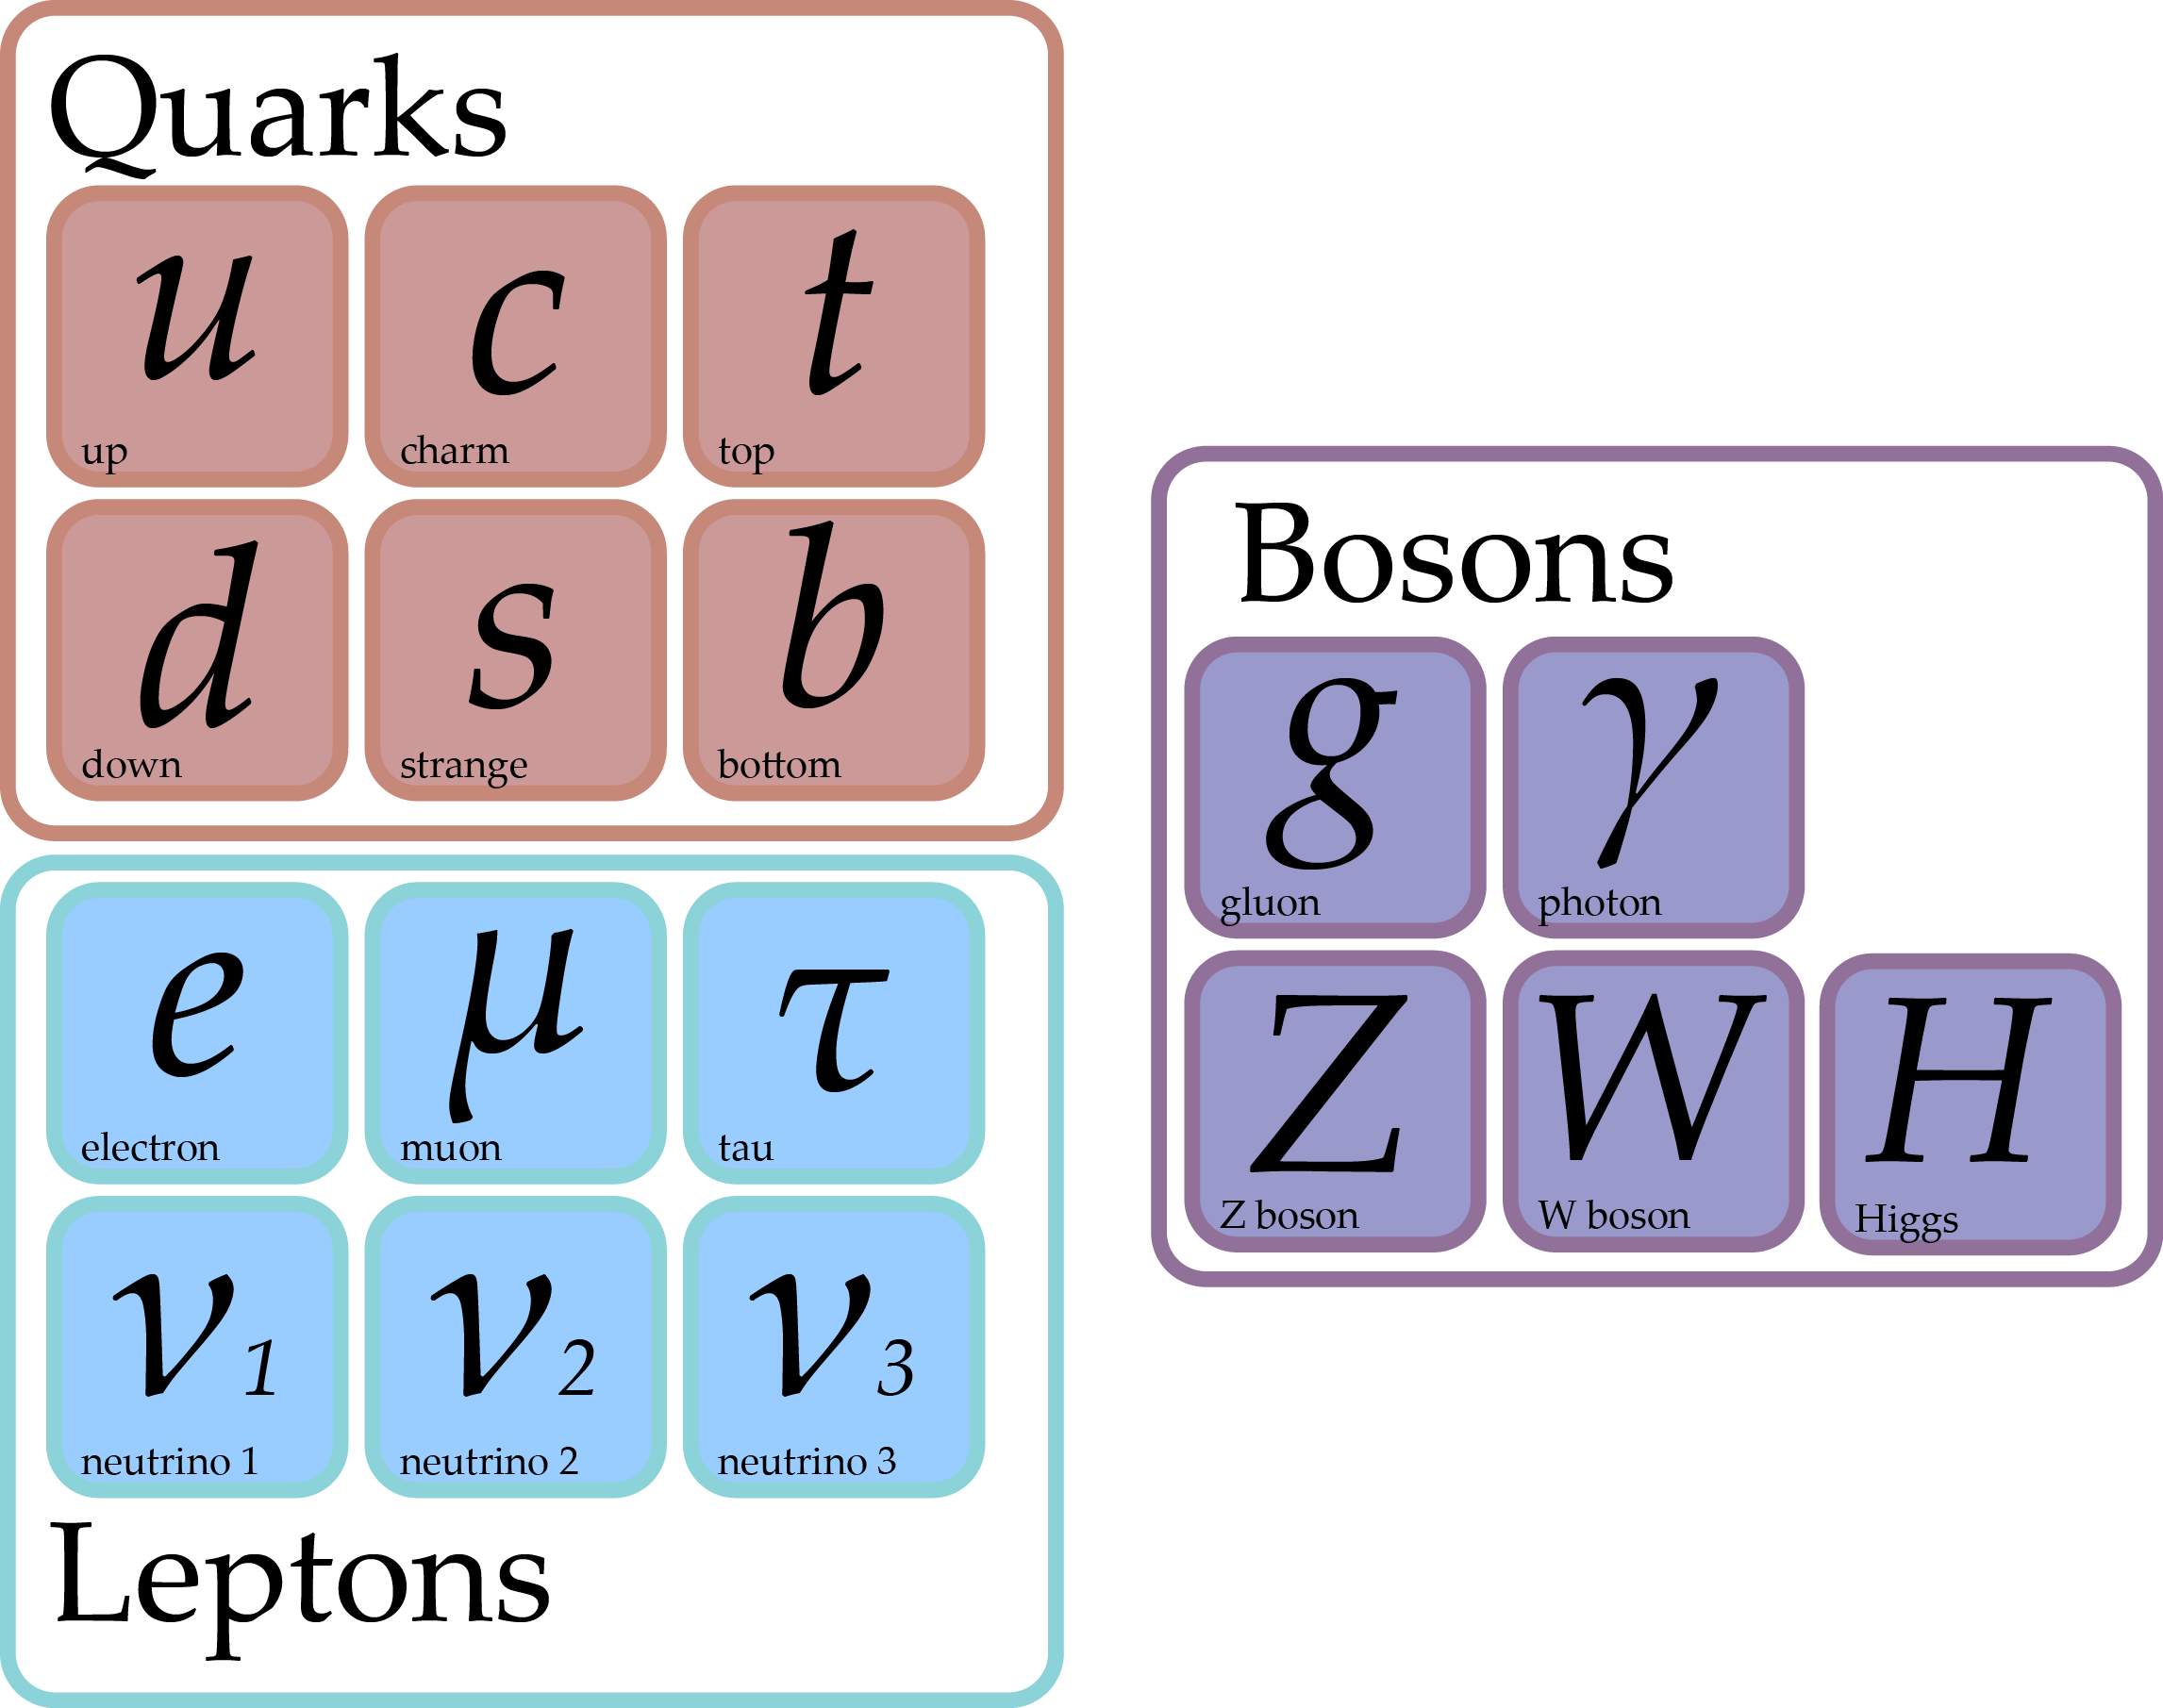
\includegraphics[width=0.8\linewidth]{figures/particles.png}
    \caption{A table of the seventeen fundamental particles. Only the mass-eigenstates for the fermions are shown.}\label{fig:party}
\end{figure}
This three-mass and three active-flavor neutrino \index{neutrino} paradigm has been well-studied~\cite{PhysRevD.98.030001,Esteban_2019,de_Salas_2018,Capozzi_2016,zboson2006, berns2021recent}, and is the conventional understanding.
At least two neutrinos are known to be massive, but as of the time of writing there exist only upper bounds on their masses, and it is uncertain by which mechanism neutrinos get their mass.

However, several anomalies persist at short baselines, including in $\nu_\mu\rightarrow\nu_e $ appearance in decay-in-flight~\cite{aguilar2018significant} and decay-at-rest~\cite{Athanassopoulos_1998} beams  and $\nu_e\rightarrow\nu_e$ disappearance at reactors~\cite{mention2011reactor,serebrov2019first}  and with $^{71}$Ga electron capture sources~\cite{PhysRevC.73.045805,giunti2011statistical}.  
These anomalies have been attributed to possible oscillations of unknown neutrinos with mass-squared differences in the range of $\Delta m^{2}\sim 0.1-10\text{ eV}^{2}$~\cite{abazajian2012light}.   
Such an additional neutrino flavor state must be non-weakly interacting, or ``sterile,'' to be consistent with observed decay widths of the Z-boson~\cite{zboson2006}; the simplest such model is known as the ``3+1'' light sterile neutrino model in which a single sterile neutrino is added. 

There have been interesting recent developments for the 3+1 model.  
The BEST experiment appears to validate the anomalous electron neutrino disappearance signature of the previous gallium anomalies with a new level of statistical significance and experimental precision~\cite{barinov2021results}. 
The Neutrino-4 experiment claims evidence of short-baseline oscillations in the $\bar{\nu}_e$ disappearance channel with $\Delta m^2\sim 7.3\,\mathrm{eV}^2$ at the 2.9$\sigma$ level.
 Meanwhile results from the MicroBooNE~\cite{microboonecollaboration2021search,microboonecollaboration2021search1,microboonecollaboration2021searchmulti} experiment challenge the interpretation that the MiniBooNE low energy excess~\cite{miniboone2018} is due entirely to the electron neutrino by placing a constraint on the sterile neutrino interpretation of the excess; though the impact of this observation on the 3+1 model has yet to be assessed.  Continued exploration of sterile neutrino mixing in all channels and all energy ranges thus remains strongly motivated~\cite{sbnfermilab}.

The addition of a fourth neutrino mass and flavor eigenstate expands the unitary mixing matrix to four dimensions. 
The four-neutrino oscillations model becomes an extension of the three-neutrino model with three additional mixing angles $\theta_{14}$, $\theta_{24}$, and $\theta_{34}$, and two new CP-violating phases $\delta_{14}$ and $\delta_{24}$. These three new mixing angles parametrize the amplitude of oscillations between the three active states and the one sterile state, and lead to additional short-baseline vacuum-like oscillations as well as novel effects in the presence of matter~\cite{Akhmedov:1988kd,KRASTEV1989341,Chizhov:1998ug, Chizhov_1999, Akhmedov_2000, Nunokawa:2003ep,Petcov:2016iiu}.  In this work we consider CP-conserving models with all CP-violating phases set to zero.

Of particular interest to neutrino telescopes, matter effects can result in the near complete disappearance of TeV-scale muon anti-neutrinos passing through the Earth's core for a sterile neutrino with eV-scale mass squared differences~\cite{Nunokawa:2003ep, Choubey:2007ji, Barger:2011rc, Esmaili:2012nz, esmaili2013restricting, Lindner:2015iaa}. This signature of matter-enhanced resonant disappearance has been targeted by the IceCube Neutrino Observatory~\cite{Aartsen_2020, Aartsen_2020_prd}, leading to one of the  most sensitive $\nu_\mu$ disappearance analyses to date. The result of the analysis was a closed 90\% contour with best fit point at $\sin^2 2\theta_{24}\sim0.1$ and $\Delta m^2_{14}=4.5\text{ eV}^2$, under a conservative assumption (for the $\nu_\mu$ disappearance channel) that $\theta_{34}=\theta_{14}=0$. In addition to being a strong refutation, lower mass solutions consistent with the LSND~\cite{Athanassopoulos_1998} and MiniBooNE anomalies and constraints around 1~eV$^2$~\cite{kopp2013sterile, Cirelli:2004cz, abazajian2012light, Gariazzo:2017fdh, Dentler:2017tkw, Diaz:2019fwt}, a possible interpretation of this result is as a statistically weak hint of a disappearance signature around $\Delta m^2_{41}\sim4.5\text{ eV}^2$.  Further exploration of this region of parameter space  in other channels at neutrino telescopes is therefore strongly motivated. 

\subsection{Neutrino oscillations}
\index{neutrino!oscillations}

First, a review of how these oscillations happen is of merit. 
For decades, now, it has been well understood that the neutrinos have multiple distinct flavor and mass eigenstates.
A consequence of this is that a neutrino prepared in a definite eigenstate will oscillate through different superpositions of its mass eigenstates, and when the flavor is measured after some time it may be observed to be in a distinct flavor eigenstate from that in which it was created. 
To understand \textit{why} that is the case we consider that there is some unitary matrix, 
\begin{equation}
    U_{\text{PMNS}} = \left(\begin{array}{ccc} U_{e1} & U_{e2} & U_{e3} \\ U_{\mu 1} & U_{\mu 2} & U_{\mu 3} \\ U_{\tau 1} & U_{\tau 2} & U_{\tau 3} \end{array}\right)
\end{equation}
which allows for rotations from the mass basis to the flavor basis, such that
\begin{equation}
    \left(\begin{array}{ccc} \nu_{e} & \nu_{\mu} & \nu_{\tau} \end{array}\right)  = \left(\begin{array}{ccc} U_{e1} & U_{e2} & U_{e3} \\ U_{\mu 1} & U_{\mu 2} & U_{\mu 3} \\ U_{\tau 1} & U_{\tau 2} & U_{\tau 3} \end{array}\right) \left(\begin{array}{c} \nu_{1} \\ \nu_{2} \\ \nu_{3} \end{array}\right).
\end{equation}
where $\nu_{i}$, $i\in\left(1,2,3\right)$ is in the mass basis and $i\in\left(e,\mu\tau\right)$ is in the flavor basis. 
This is called the Pontecorvo-Maki-Nakagawa-Sakata (PMNS) matrix.
We can, in general then, express a stationary state in the flavor basis in terms of the mass basis:
\begin{equation}\label{eq:nunu}
    \ket{\nu_{e}} = U_{e1} \ket{\nu_{1}} + U_{e2} \ket{\nu_{2}} + U_{e3}\ket{\nu_{3}}.
\end{equation}
To consider a neutrino in-flight, we consider the time-dependent Schr\"odinger Equation
\begin{equation}
    i\dfrac{\partial}{\partial t} \ket{\nu_{i} (t)} = \bvec{H}_{\nu}\ket{\nu_{i}(t)},
\end{equation}
which can be solved with the stationary state solution 
\begin{equation}
    \ket{\nu_{i} (t)}  =  e^{-iEt} \ket{\nu_{i} (0)}.
\end{equation}
For neutrinos, we can expand out the energy term and simplify under the small-mass assumption. 
\begin{align}
    E_{i} &= \sqrt{p^{2}c^{2} + m_{i}^{2}c^{4}} \\
    &\approxeq pc + \dfrac{m_{i}^{2}c^{4}}{2E}
\end{align}
The stationary state solution then becomes, using $t=L/c$ and $c=1$ 
\begin{equation}
    \ket{\nu_{i} (t)}  =  e^{-ipt}e^{ -m_{i}^{2}L/2E}\ket{\nu_{i} (0)}
\end{equation}
and for the state described in Equation~\eqref{eq:nunu},

\begin{equation}
    \ket{\nu_{e}(t)} = \sum\limits_{i} U_{ei} e^{-ipt}e^{ -m_{i}^{2}L/2E}\ket{\nu_{i} (0)}
\end{equation}

Oscillations probabilities can be calculated by projecting the final considered state onto this propagated state


\begin{equation}
    \braket{\nu_{\mu} | \nu_{e}(t)} = e^{-ipt} \sum\limits_{i} U_{\mu i}^{*}U_{ei} e^{ -m_{i}^{2}L/2E}
\end{equation}
To calculate actual transmission probabilities, we need the conjugate squared of this, $P_{e\mu} = \left|\braket{\nu_{\mu}|\nu_{e}(t)}\right|^{2}$. While the phase term, $e^{-ipt}$, cancels we are left with 
\begin{equation}\begin{split}
P_{\mu e}&= \sum\limits_{i}\left[\left|U_{\mu i}\right|^{2}\left|U_{e i}\right|^{2} \right.\\
&\hspace{1cm} + 2\sum\limits_{i>j}U_{\mu i}^{*}U_{e i}U_{\mu j}U_{e j}^{*}\left.e^{-i\Delta m_{ij}^{2}L/2E} \right]
\end{split}\end{equation} 
Using the sinusoidal form of the exponential, we can write this in other components 
\begin{equation}\begin{split}
    P_{\mu e}&= \sum\limits_{i}\left[\left|U_{\mu i}\right|^{2}\left|U_{e i}\right|^{2} \right.\\
    &\hspace{1cm} -2\sum\limits_{i>j} \Re(U_{\mu i}^{*}U_{e i}U_{\mu j}U_{e j}^{*})\cos\left(\Delta m_{ij}^{2}L/2E \right) \\
    &\hspace{1cm} -2\sum\limits_{i>j}\Im(U_{\mu i}^{*}U_{e i}U_{\mu j}U_{e j}^{*})\sin\left(\Delta m_{ij}^{2}L/2E \right)
\end{split}\end{equation} 

From this we notice a few things. 
Neutrino oscillation probabilities are dependent not just on the mass of the neutrino eigenstates, but the differences of square of the masses. 
Through oscillations we can only measure the absolute of the difference of the masses, and so the ordering of the masses will be invisible to oscillations. 
This also suggests that, since oscillations have been observed, at minimum two of the neutrino masses must be non-zero. 
Oscillations will also depend on the energy $E$ of the neutrinos involved and the baseline $L$ over which they travel. \index{neutrino!baseline}

\subsection{Higher Neutrino Numbers}

In general, we can relate a flavor and mass eigenstates by 
\begin{equation}
    \braket{\nu_{\alpha}} = \sum_{i} U_{\alpha i}^{*}\braket{\nu_{i}}
\end{equation}
where $U$ is the neutral lepton mixing matrix.
For antineutrinos the relation is the same, although $U\to U^{*}$. 
In the cases with a number of neutrinos greater than three, we parametrize $U$ as a product of complex rotations parametrized by angles $\theta_{ij}$ and phases $\delta_{ij}$, 
\begin{equation}
    U(\theta_{ij}, \delta_{ij}) = R_{N-1,N}R_{N-2,N}\ldots R_{45}R_{34}R_{24}R_{15}R_{34}R_{24}R_{14}R_{23}R_{13}R_{12}
\end{equation}
as discussed in Ref~\cite{Arguelles:2020hss}

\subsection{Neutrino Interactions}
\index{neutrino!interactions}
Discuss neutrino interactions at medium to high energies. Deep Inelastic Scattering


\subsection{Matter Effects on Neutrion Oscillations}
\index{neutrino!matter effect}
Neutrinos propagating in the presence of matter will experience a coherent forward elastic scattering with electrons and nucleons in the medium through which they propagate. Although all three neutrinos can scatter via Z$^{0}$ boson exchange with nucleons only $\nu_{e}$ can scatter via the exchange of W$^{\pm}$ and Z$^{0}$ with electrons. 
The consequence of these interactions is that neutrinos behave as if they had slightly different masses, which are referred to as effective massses, and so their oscillations are impacted.  
Mathematically, in the two-neutrino case the total effective Hamiltonian governing the neutrino propagation is modified via the orgogonal matrix 
\begin{equation}
    U^{m} = \left( \begin{array}{cc} \cos\theta^{m} & \sin\theta^{m} \\ -\sin\theta^{m} & \cos\theta^{m} \end{array}\right) 
\end{equation}


\section{Passage of Particles through Matter}

\subsection{Cherenkov Radiation}

High enough energy particles passing through matter are capable of moving faster than light in the medium. 

\begin{equation}
    E^{2} = m^{2} + p^{2}
\end{equation}

we can substitute in the relativistic formulation of momentum
\begin{equation}
    p = \dfrac{mv}{\sqrt{1-v^{2}}}
\end{equation}

and so the energy-velocity relation takes the form 
\begin{equation}
    E^{2} = m^{2} + \dfrac{m^{2}v^{2}}{1-v^{2}}
\end{equation}
Consider a material with index of refraction $n = 1./v_{critical}$, where $v$ is the phase velocity light in the medium. 
Particles travelling at this speed above which particles will emit Cherenkov radiation. 
The associated energy $E_{critical}$ can be solved for algebraically,
\begin{align}
        E^{2}_{critical} &= m^{2} + \dfrac{m^{2}v_{critical}^{2}}{1-v_{critical}^{2}} \\
        E^{2}_{critical}  - m^{2} - E^{2}_{critical}v_{critical}^{2}  + m^{2}v_{critical}^{2} &= m^{2}v_{critical}^{2} \\
        E^{2}_{critical}\left(1  -v_{critical}^{2}\right) &=  m^{2} \\
        \sqrt{\dfrac{m^{2}}{\left(1  -n^{-2}\right)}} &= E_{critical} 
\end{align}

Like a sonic boom of light, the Cherenkov light is emitted in a cone at an angle $\theta_{c}$ relative to the direction a particle traveling at velocity $v$ is moving, and is given by
\begin{equation}
\tan\theta_{c} = \sqrt{v^{2}n^{2} - 1} 
\end{equation}
Although the light is emitted in the forward direction, the Cherenkov light wave-front counter-intuitively trails in a cone opening behind the radiating particle. 

The rate of energy loss 
\begin{equation}
-\left(\dfrac{dE}{dx}\right) =\left(2\pi e\right)^{2}\int \left(1-\dfrac{1}{\left(vn\right)^{2}}\right)\nu d\nu
\end{equation}

\subsection{Neutrino Propagation}
In addition to neutirno oscillation, several other phenomena effect the full description of the neutrino flux as it propagates through the Earth. 
These include, but are not limited to, neutrino flux attenuation as neutrinos interact in the Earth, the process where charged tau leptons produced through neutrino-nucleon interactions decay to produce lower energy tau neutrinos called tau regeneration, and Glashow resonance interactions~\cite{PhysRev.118.316}.  

This section  describes the methods of determining propagation of neutrino fluxes from Earth-surface fluxes to in-IceCube fluxes. 
Here, we summarize the procedures described also in Reference~\cite{arguelles2021nusquids}.

The neutrino flux is described as a function of energy $E$ and location $x$ for neutrino flavor $\alpha$ using the density matrix formalism in the weak-interaction flavor-eigenstate basis as 
\begin{equation}
    \rho(E,x) = \sum_{\alpha} \phi_{\alpha}(E,x) \ket{\nu_{\alpha}}\bra{\nu_{\alpha}}.
\end{equation}
where $\phi_{\alpha}$ specifies the neutrino flux of the flavor $\alpha$. 
The evolution of the system is described by the von Neumann equation
\begin{equation}\label{eq:evol}
    \dfrac{\partial\rho (E,x)}{\partial x} = -i\left[ H(E,x), \rho(E,x)\right],
\end{equation}
where $H$ is the Hamiltonian for the whole system. 
$H$ can be approximated, in the case of small perturbations, as
\begin{equation}
    H(E,x) = H_{0}(E) + H_{1}(E,x)
\end{equation}
where $H_{0}$ is the term giving vacuum neutrino oscillations, which can be solved exactly, and $H_{1}$ is an additional term incorporating matter-effects.
These are, for neutrinos,
\begin{align}
    H_{0}(E) &= \dfrac{1}{2E} \left(\begin{array}{ccc} 0 & 0 & 0\\ 0 & \Delta m_{21}^{2} & 0 \\ 0 & 0 & \Delta m_{31}^{2}\end{array}\right)  \\
    H_{1}(E,x) &= \sqrt{2}G_{F} N_{e}(x) U_{PMNS}^{\dag} \left(\begin{array}{ccc}1&0&0 \\ 0 &0 & 0 \\ 0 & 0 & 0 \end{array}\right) U_{PMNS},
\end{align}
where $G_{F}$ is the Fermi constant, $U_{PMNS}$ is the PMNS neutrino mixing matrix, $N_{e}$ is the electron number density at position $x$, and the $\Delta m^{2}$ terms are the mass-squared splittings.  
Since the evolution of the vacuum component can be soled analytically, it is more convenient to evolve of the system in the interaction basis. 
So, we transform the density matrix and the mass-effect terms as 
\begin{align}
    \rho_{1}(E,x) &= e^{-i H_{0}x}\rho(E,x) e^{-iH_{0}x}. \\
    H_{I,1}(E,x)&= e^{-i H_{0}x} H_{1}(E,x) e^{-iH_{0}x}.
\end{align}
Similarly to Equation~\eqref{eq:evol}, the evolution in the interaction basis is dependent on the matter-effect term,
\begin{equation}\label{eq:mattermod}
    \dfrac{\partial_{1}\rho (E,x)}{\partial x} = -i\left[ H_{I,1}(E,x), \rho(E,x)\right].
\end{equation}
We require a series of additional terms that modify Eq~\eqref{eq:mattermod} to account for the effects which do not preserve neutrino number and energy. 
The first of which is the attenuation of the fluxes from neutrino-Earth interactions, which follow 
\begin{align}\label{eq:nu_evol}
    \Gamma(E,x) &= \dfrac{1}{2}\sum\limits_{\alpha\in(e,\mu,\tau)} \dfrac{\Pi_{\alpha}(E,x) }{\lambda_{NC}^{\alpha}(E,x) + \lambda_{CC}^{\alpha} (E,x)} \\
    \bar{\Gamma}(E,x) &= \dfrac{1}{2}\sum_{\alpha\in(e,\mu,\tau)} \dfrac{\bar{\Pi}_{\alpha(E,x)}}{\bar{\lambda}_{NC}^{\alpha}(E,x) + \bar{\lambda}_{CC}^{\alpha}(E,x) + \bar{\lambda}_{GR}^{\alpha}(E,x) }\label{eq:nubar_evol}
\end{align}
where $\Pi_{\alpha}$ is a neutrino projector onto the flavor $\alpha\in\left\lbrace e,\mu\tau\right\rbrace$, $\nu_{CC}^{\alpha}$ ($\nu_{NC}^{\alpha}$) is the charged (neutral) current neutrino interaction length given by $1/\left[ N_{nuc}(x)\sigma^{\alpha}_{CC(NC)}(E) \right]$~\cite{Formaggio:2013kya, Gandhi:1995tf, Beacom:2019pzs, Zhou:2019vxt, Cooper_Sarkar_2011}, and $\bar{\lambda}_{GR}^{e}$ is the mean free path due to the Glashow Resonance $1/\left[ N_{e}(x)\sigma^{e}_{GR}(E) \right]$~\cite{PhysRev.118.316}. 

We also account for tau regeneration, neutrino-antineutrino coupling, and low-energy neutrino re-injection from neutral current interactions following the functional forms for neutrinos $F$ and antineutrinos $\bar{F}$ given by 
\begin{equation}\begin{split}
    F\left[\rho,\bar{\rho}, E, x\right] &= \sum\limits_{\alpha} \Pi_{\alpha}(E,x)\int\limits_{E}^{\infty}\dfrac{\text{Tr}\left[ \Pi(E_{\nu_{\alpha}},x)\rho(E_{\nu_{\alpha}}, x) \right]}{\lambda_{NC}^{\alpha}(E_{\nu_{\alpha}}, x) } \dfrac{\partial N_{NC}^{\alpha}(E_{\nu_{\alpha}}, E)}{\partial E} dE_{\nu_{\alpha}} \\ 
    &+\Pi_{\tau}(E,x) \int\limits_{E}^{\infty}\int\limits{E_{\tau}}^{\infty} \dfrac{\text{Tr}\left[ \Pi(E_{\nu_{\tau}},x)\rho(E_{\nu_{\tau}}, x) \right]}{\lambda_{NC}^{\tau}(E_{\nu_{\tau}}, E) } \dfrac{\partial N_{NC}^{\tau}(E_{\nu_{\tau}}, x)}{\partial E} \\
    &\times \dfrac{\partial N_{dec}^{all}(E_{\tau}, E)}{\partial E} dE_{\nu_{\tau}}dE_{\tau} \\
    &+\left[ \text{Br}\left(\tau^{-} \to \bar{\nu}_{e}\right)\Pi_{e}(E,x)\int\limits_{E}^{\infty}\int\limits_{E_{\tau}}^{\infty} \dfrac{\text{Tr}\left[ \bar{\Pi}(E_{\nu_{\tau}},x)\bar{\rho}(E_{\nu_{\tau}}, x) \right]}{\bar{\lambda}_{NC}^{\tau}(E_{\bar{\nu}_{\tau}}, x) }\right.  \\
    &+ \left. \text{Br}\left(\tau^{-} \to \bar{\nu}_{\mu}\right)\Pi_{\mu}(E,x)\int\limits_{E}^{\infty}\int\limits_{E_{\tau}}^{\infty} \dfrac{\text{Tr}\left[ \bar{\Pi}(E_{\nu_{\tau}},x)\bar{\rho}(E_{\nu_{\tau}}, x) \right]}{\bar{\lambda}_{NC}^{\tau}(E_{\bar{\nu}_{\tau}}, x) } \right] \\
    &\times \dfrac{\partial \bar{N}_{CC}^{\tau}(E_{\bar{\nu}_{\tau}}, E)}{\partial E} \dfrac{\partial\bar{N}_{dec}^{lep} (E_{\tau}, E)}{\partial E} dE_{\bar{\nu}_{\tau}} dE_{\tau}
\end{split}\end{equation}
and 
\begin{equation}\begin{split}
    \bar{F}\left[\rho,\bar{\rho}, E, x\right] &= \sum\limits_{\alpha}\bar{\Pi}_{\alpha}(E,x)\int\limits_{E}^{\infty}\dfrac{\text{Tr}\left[ \bar{\Pi}(E_{\bar{\nu}_{\alpha}}, x) \bar{\rho}(E_{\bar{\nu}_{\alpha}}, x) \right]}{\bar{\lambda}_{NC}^{\alpha}(E_{\bar{\nu}_{\alpha} }, x)}\dfrac{\partial\bar{N}_{NC}^{\alpha}(E_{\bar{\nu}_{\alpha}}, E)}{\partial E} d E_{\bar{\nu}_{\alpha}} \\ 
    &+ \bar{\Pi}_{\tau} (E,x) \int\limits_{E}^{\infty}\int\limits_{E_{\tau}}^{\infty}\dfrac{\text{Tr}\left[ \bar{\Pi}(E_{\bar{\nu}_{\tau}}, x) \bar{\rho}(E_{\bar{\nu}_{\tau}}, x) \right]}{\bar{\lambda}_{NC}^{\tau}(E_{\bar{\nu}_{\tau} }, x)}\dfrac{\partial\bar{N}_{NC}^{\tau}(E_{\bar{\nu}_{\tau}}, E)}{\partial E} \\
    &\times \dfrac{\partial\bar{N}_{dec}^{all}(E_{\tau}, E)}{\partial E} dE_{\bar{\nu}_{\tau}} dE_{\tau} \\
    &+ \left[ \text{Br}\left(\tau^{+} \to \nu_{e}\right)\bar{\Pi}_{e}(E,x)\int\limits_{E}^{\infty}\int\limits_{E_{\tau}}^{\infty} \dfrac{\text{Tr}\left[\Pi(E_{\nu_{\tau}}, x)\rho(E_{\nu_{\tau}}, x) \right] }{\lambda_{NC}^{\tau}(E_{\nu_{\tau}}, x)}  \right. \\
    &+ \left.\text{Br}\left(\tau^{+} \to \nu_{\mu}\right)\bar{\Pi}_{\mu}(E,x)\int\limits_{E}^{\infty}\int\limits_{E_{\tau}}^{\infty} \dfrac{\text{Tr}\left[\Pi(E_{\nu_{\tau}}, x)\rho(E_{\nu_{\tau}}, x) \right] }{\lambda_{NC}^{\tau}(E_{\nu_{\tau}}, x)}  \right] \\
    &\times \dfrac{\partial N_{CC}^{\tau}(E_{\nu_{\tau}}, E)}{\partial E} \dfrac{\partial N_{dec}^{lep}(E_{\tau}, E)}{\partial E} dE_{\nu_{\tau}} dE_{\tau} \\
    &+\left(\sum\limits_{\alpha} \bar{\Pi}_{\alpha} (E,x)\right) \int\limits_{E}^{\infty} \dfrac{\text{Tr}\left[\bar{\Pi}_{e}(E_{\bar{\nu}_{e}}, x) \bar{\rho}(E_{\bar{\nu}_{e}}, x) \right]}{\bar{\lambda}_{GR}^{e} (E_{\bar{\nu}_{e}}, x)}  \\
    &\times \dfrac{\partial\bar{N}_{GR}^{e}(E_{\bar{\nu}_{e}}, E)}{\partial E} dE_{\bar{\nu}_{e}}
\end{split}\end{equation}

Interaction rates in these functionals for neutral current, charged current, and Glashow resonance interactions are given by 

\begin{align}
    \dfrac{\partial N_{NC(CC)}^{\tau} (E_{\nu_{\tau}}, E)}{\partial E} &= \dfrac{1}{\sigma_{NC(CC)}^{\alpha} (E_{\nu_{\alpha} })}\dfrac{\partial\sigma_{NC(CC)}^{\alpha}(E_{\nu_{\alpha}}, E_{\alpha})}{\partial E_{\alpha}}\hspace{0.5cm} \text{ and}, \\
    \dfrac{\bar{N}_{GR}^{e} (E_{\bar{\nu}_{e}}, E)}{\partial E} &= \dfrac{1}{\sigma_{GR}^{e}(E_{\bar{\nu}_{e}})} \dfrac{\partial\sigma_{GR}^{e}(E_{\bar{\nu}_{e}}, E_{e})}{\partial E}.
\end{align}
The tau decay distributions for the leptonic-only modes ($N_{dec}^{lep}$) and for all-modes ($N_{dec}^{all}$) are given by 
\begin{align}
    \dfrac{\partial N_{dec}^{lep}(E_{\tau}, E)}{\partial E} &= \dfrac{1}{\bar{\Gamma}_{lep}^{\tau}(E_{\tau})} \dfrac{\partial\bar{\Gamma}_{lep}^{\tau}(E_{\tau},E)}{\partial E} \\
    \dfrac{\partial N_{dec}^{all}(E_{\tau}, E)}{\partial E} &= \dfrac{1}{\bar{\Gamma}_{all}^{\tau}(E_{\tau})} \dfrac{\partial\bar{\Gamma}_{all}^{\tau}(E_{\tau},E)}{\partial E} 
\end{align}

These systems are implemented within the \texttt{nuSQuIDS} framework~\cite{arguelles:2015nu, arguelles2021nusquids}, which implements Equations~\eqref{eq:nu_evol}-\eqref{eq:nubar_evol} to numerically propagate the state-density matrix along a neutrino fluxes' baseline. 
Different neutrino oscillation parameters can be specified, along with various other new physics scenarios, if desired.
\end{document}
